\begin{frame}{Valorisation des archives de Jean-Martin Charcot}
\vspace{-3ex}
       \begin{table}[h]
\begin{tabular}{|c|}
\hline
\fontsize{9}{10}\selectfont \textit{Dans les petits papiers de Charcot : de l'expérimentation aux prémisses de la neurologie moderne\footnote{\url{https://theses.fr/s382733}}} \\ \hline
\end{tabular}
\end{table}
    \begin{columns}
    \column{0.53\textwidth}
    CS en linguistique (2019-)\\
    \begin{itemize}
    \footnotesize
    \item directeur : Prof. D\textsuperscript{r} Christopher LAENZLINGER
    \item co-directeur : Luka NERIMA
    \end{itemize}
       Thèse en cours (2021-)
%       \scriptsize \centering \textit{Dans les petits papiers de Charcot : de l'expérimentation aux prémisses de la neurologie moderne}
       \begin{itemize}
       \footnotesize
       \item directeur : Prof. D\textsuperscript{r} Glenn ROE
       \item co-encadrant : D\textsuperscript{r} Motasem ALRAHABI
       \end{itemize}

    \column{0.47\textwidth}
        \begin{figure}
        \centering
        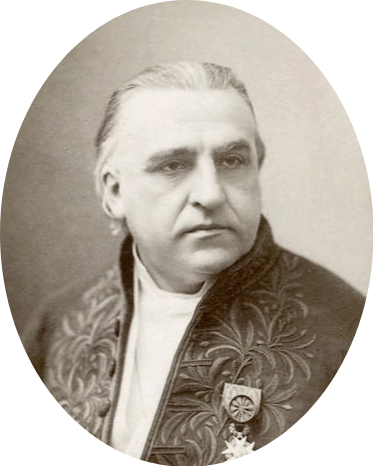
\includegraphics[width=.2\textwidth]{pic/Jean-Martin_Charcot-modified.png}
        \caption{J.-M. Charcot (1825-1893) (\href{https://fr.wikipedia.org/wiki/Jean-Martin_Charcot\#/media/Fichier:Jean-Martin\_Charcot.jpg}{Wikipédia}).}
        \end{figure}
        \begin{itemize}
        \small
        \item Père de la neurologie moderne
        \item Impact sur son \og{}réseau\fg{} \\
         {\footnotesize $\quad$Freud, de la Tourette, Babinski$\dots$
         }
        \item hystérie, SLA, Parkinson$\dots$
        \item Fonds Charcot sur SorbonNum\footnote{\url{https://patrimoine.sorbonne-universite.fr}}
%        \item Corpus Charcot sur \textsc{OBVIE}\footnote{\url{https://obtic.huma-num.fr/obvie/charcot/?view=corpus}}
        \end{itemize}
    \end{columns}
    
%    \begin{exampleblock}{}
%\centering
%    \color{deepblue}{\textmd{\textcolor{purple}{Pister numériquement la circulation du discours médical de Charcot}}}
%\end{exampleblock}

    

\end{frame}